\documentclass[conference]{IEEEtran}
\usepackage{algorithm}
\usepackage{algpseudocode}
\usepackage{listings}
\usepackage{xcolor}
\usepackage{amsmath}
\usepackage{graphicx}
\usepackage{float}
\usepackage{booktabs}
\usepackage{url}
\usepackage{circuitikz}
\lstset{
  basicstyle=\ttfamily\small,
  keywordstyle=\color{blue}\bfseries,
  commentstyle=\color{green!40!black},
  stringstyle=\color{red},
  numbers=left,                     % keep numbers
  numberstyle=\scriptsize\ttfamily, % more readable numbers
  numbersep=8pt,                    % add spacing from code
  xleftmargin=1.5em,                % indent code so numbers don’t overlap
  frame=single,
  breaklines=true,
  breakatwhitespace=true,
  tabsize=2,
  showstringspaces=false,
  captionpos=b,
  keepspaces=true                   % preserve spacing properly
}

\title{Implementation of Scientific Calculator Functions on Microcontroller using C}

\author{
\IEEEauthorblockN{Krishna Patil, Nara Prajwal}
\IEEEauthorblockA{
Department of Electrical Engineering\\
IIT Hyderabad\\
Email: ee24btech11036@iith.ac.in, ee24btech11051@iith.ac.in}
}

\begin{document}

\maketitle

\begin{abstract}
This paper presents the implementation of scientific calculator functions such as trigonometric, logarithmic, exponential, power, factorial, and expression parsing using the C programming language on a microcontroller platform. Various numerical algorithms such as Runge--Kutta (RK4), series expansions, iterative methods, and parsing algorithms have been employed. Each function is discussed with its algorithmic basis followed by its C implementation.
\end{abstract}

\begin{IEEEkeywords}
Scientific Calculator, Microcontroller, Runge--Kutta Method, Quake III Algorithm, Shunting Yard Algorithm, C Programming
\end{IEEEkeywords}

\section{Software Implementation}

Instead of using "general expansion methods" (like Taylor/Maclaurin series with many terms), we reformulated each function as a differential equation.
 The algorithms used to calculate the values are  RK4 (for ODEs), Newton–Raphson (for refinements like inverse sqrt).

\subsection{Supported Functions}

\begin{table}[htbp]
\centering
\caption{Supported Functions and Operations}
\label{tab:supported}
\begin{tabular}{ll}
\toprule
\textbf{Category} & \textbf{Functions / Operations} \\
\midrule
Trigonometric & $\sin(x), \cos(x), \tan(x)$ \\
Inverse Trigonometric & $\arcsin(x), \arccos(x), \arctan(x)$ \\
Exponential / Logarithmic & $e^x, \ln(x)$ \\
Power / Root & $x^y, \tfrac{1}{\sqrt{x}}$ \\
Factorial & $n!$ \\
Basic Arithmetic & $+, -, \times, \div$ \\
Constants & $\pi, e$ \\
Input Symbols & Digits $0$–$9$, decimal point, parentheses $(,)$ \\
\bottomrule
\end{tabular}
\end{table}

\subsection{Runge--Kutta Method (RK4)}
We employ the fourth-order Runge--Kutta (RK4) method \cite{grewal2014,kreyszig2011} 
to solve ordinary differential equations for trigonometric and exponential functions.
The full derivation and step-by-step procedure are provided in Appendix~\ref{appendix:rk4}.

\subsection{Trigonometric Functions}

\subsubsection{Sine Function} 
The sine function \cite{ncert12} is computed by solving the second-order differential equation:
\begin{align}
\frac{d^2y}{dx^2} + y = 0, \quad y(0)=0, \quad y'(0)=1
\end{align}
using the fourth-order Runge--Kutta method.

System:
\begin{align}
\frac{dy}{dx}=z, \quad \frac{dz}{dx}=-y, \quad y(0)=0, \; z(0)=1
\end{align}

The $ k_1,k_2,k_3,k_4 $ corresponds to the RK-4 terms of the equation $ \frac{dy}{dx}=z $ and the $ l_1,l_2,l_3,l_4 $ corresponds to the RK-4 terms of the equation $ \frac{dz}{dx}=-y $

RK4 step values:
\begin{align}
k_1 &= h z_n, \\
l_1 &= -h y_n, \\
k_2 &= h \left(z_n+\tfrac{l_1}{2}\right), \\
l_2 &= -h \left(y_n+\tfrac{k_1}{2}\right), \\
k_3 &= h \left(z_n+\tfrac{l_2}{2}\right), \\
l_3 &= -h \left(y_n+\tfrac{k_2}{2}\right), \\
k_4 &= h(z_n+l_3), \\
l_4 &= -h(y_n+k_3), \\
y_{n+1} &= y_n+\frac{1}{6}(k_1+2k_2+2k_3+k_4), \\
z_{n+1} &= z_n+\tfrac{1}{6}(l_1+2l_2+2l_3+l_4).
\end{align}

\subsubsection{Cosine Function} 
The cosine function \cite{ncert12} is computed by $\sin(\frac{\pi}{2} - x)$ .



\subsubsection{Tangent Function} 
Tangent \cite{ncert12} is implemented as the ratio of sine and cosine:

\subsection{Inverse Square Root}

\subsubsection{Inverse Square Root}
The fast inverse square root algorithm (Quake III method) is used to efficiently compute $x^{-1/2}$. 
Detailed derivation and Newton–Raphson refinement are included in Appendix~\ref{appendix:inv_sqrt}.

\subsection{Inverse Trigonometric Functions}
\subsubsection{Arcsine} 
The ODE for the arcsine function \cite{ncert12} is
ODE:
\begin{align}
\frac{dy}{dx} = \frac{1}{\sqrt{1-x^2}}, \quad y(0)=0
\end{align}

\subsubsection{Arccosine}
 Use the identity \cite{ncert12}
\begin{align}
   \arccos(x) = \frac{\pi}{2} - \arcsin(x) 
\end{align}

\subsubsection{Arctangent}
The ODE for the arctan function \cite{ncert12} is
ODE:
\begin{align}
\frac{dy}{dx} = \frac{1}{1+x^2}, \quad y(0)=0
\end{align}



\subsection{Logarithmic Functions}

The natural logarithm can be obtained by solving the differential equation \cite{ncert12}
\begin{align}
\frac{dy}{dx} = \frac{1}{x}, \quad y(1)=0
\end{align}
which has the exact solution $y(x)=\ln(x)$. Using the RK4 method, we can approximate $\ln(x)$ by integrating this ODE from $x=1$ to the target value.

\subsection{Exponential Functions}

\subsubsection{Power Function} 
The power function $y=x^w$ \cite{ncert12} satisfies
\begin{align}
\frac{dy}{dx} = \frac{w}{x}y, \quad y(1)=1
\end{align}



\subsection{Factorial Function}

The algorithm is a simple recursive function in C

\begin{align}
y_n = n \cdot y_{n-1}
\end{align}

\cite{GVVSharma}

\begin{algorithm}
\caption{Recursive Factorial Function}
\begin{algorithmic}[1]
\Function{FactorialRecursive}{x}
    \If{$x \leq 1$}
        \State \Return $1$
    \Else
        \State \Return $x \times \text{FactorialRecursive}(x-1)$
    \EndIf
\EndFunction
\end{algorithmic}
\end{algorithm}

\begin{table*}[htbp]
\centering
\caption{RK4 Update Equations for Single-Variable Functions}
\label{tab:rk4_single}
\renewcommand{\arraystretch}{1.4}
\setlength{\tabcolsep}{6pt}
\begin{tabular}{lccccc}
\toprule
\textbf{Function} & \textbf{$k_1$} & \textbf{$k_2$} & \textbf{$k_3$} & \textbf{$k_4$} & \textbf{$y_{n+1}$} \\
\midrule

Arcsine $\arcsin(x)$ &
$\tfrac{h}{\sqrt{1-x_n^2}}$ &
$\tfrac{h}{\sqrt{1-(x_n+\tfrac{h}{2})^2}}$ &
$\tfrac{h}{\sqrt{1-(x_n+\tfrac{h}{2})^2}}$ &
$\tfrac{h}{\sqrt{1-(x_n+h)^2}}$ &
$y_n+\tfrac{1}{6}(k_1+2k_2+2k_3+k_4)$ \\

\midrule

Arctangent $\arctan(x)$ &
$\tfrac{h}{1+x_n^2}$ &
$\tfrac{h}{1+(x_n+\tfrac{h}{2})^2}$ &
$\tfrac{h}{1+(x_n+\tfrac{h}{2})^2}$ &
$\tfrac{h}{1+(x_n+h)^2}$ &
$y_n+\tfrac{1}{6}(k_1+2k_2+2k_3+k_4)$ \\

\midrule

Natural Log $\ln(x)$ &
$\tfrac{h}{x_n}$ &
$\tfrac{h}{x_n+\tfrac{h}{2}}$ &
$\tfrac{h}{x_n+\tfrac{h}{2}}$ &
$\tfrac{h}{x_n+h}$ &
$y_n+\tfrac{1}{6}(k_1+2k_2+2k_3+k_4)$ \\

\midrule

Power $y=x^w$ &
$h \cdot \tfrac{w}{x_n}y_n$ &
$h \cdot \tfrac{w}{x_n+\tfrac{h}{2}}\left(y_n+\tfrac{k_1}{2}\right)$ &
$h \cdot \tfrac{w}{x_n+\tfrac{h}{2}}\left(y_n+\tfrac{k_2}{2}\right)$ &
$h \cdot \tfrac{w}{x_n+h}\left(y_n+k_3\right)$ &
$y_n+\tfrac{1}{6}(k_1+2k_2+2k_3+k_4)$ \\

\bottomrule
\end{tabular}
\end{table*}

\subsection{Expression Parsing}

The Shunting Yard algorithm is employed for converting infix expressions into postfix form for evaluation.

\subsection{Overview}
The \textbf{Shunting Yard Algorithm}, proposed by Edsger Dijkstra, is a method for converting mathematical expressions in infix notation into postfix notation (Reverse Polish Notation, RPN).  
It relies on two structures:
\begin{itemize}
    \item A \textbf{stack} for operators/functions
    \item An \textbf{output queue} for the final postfix expression
\end{itemize}

\subsection{Algorithm Steps}
\begin{enumerate}
    \item Initialize an empty stack and output queue.
    \item For each token:
    \begin{enumerate}
        \item Numbers $\rightarrow$ add to output.
        \item Functions $\rightarrow$ push to stack.
        \item Operators $\rightarrow$ pop higher/equal precedence operators from stack to output (respecting associativity), then push current operator.
        \item ``('' $\rightarrow$ push to stack.
        \item ``)'' $\rightarrow$ pop to output until matching ``('' is found, discard brackets.
    \end{enumerate}
    \item After processing, pop remaining operators to output.
\end{enumerate}

\begin{algorithm}
\caption{Shunting Yard Algorithm (Infix to Postfix)}
\begin{algorithmic}[1]
\Function{ShuntingYard}{expr}
    \State Initialize empty stack $operators$
    \State Initialize empty string $output$
    \For{each character $c$ in $expr$}
        \If{$c$ is a number or '.'}
            \State Append $c$ to $output$ until number ends
            \State Append space to $output$
        \ElsIf{$c$ is a function}
            \State Push $c$ onto $operators$
        \ElsIf{$c = ($}
            \State Push $c$ onto $operators$
            \State Increment $unmatched\_brackets$
        \ElsIf{$c = )$}
            \While{Top of $operators \neq ($}
                \State Pop from $operators$ and append to $output$
            \EndWhile
            \State Pop '(' from $operators$
            \State Decrement $unmatched\_brackets$
            \If{Top of $operators$ is a function}
                \State Pop function and append to $output$
            \EndIf
        \ElsIf{$c$ is an operator in $\{+,-,*,/,^,!\}$}
            \While{$operators$ not empty \textbf{and} 
                   precedence(Top of $operators$) $\geq$ precedence($c$)}
                \State Pop from $operators$ and append to $output$
            \EndWhile
            \State Push $c$ onto $operators$
        \EndIf
    \EndFor
    \While{$operators$ not empty}
        \State Pop from $operators$ and append to $output$
    \EndWhile
    \State \Return $output$
\EndFunction
\end{algorithmic}
\end{algorithm}

\subsection{Operator Precedence}
\begin{table}[htbp]
\centering
\caption{Operator Precedence and Associativity}
\label{tab:precedence}
\begin{tabular}{lcc}
\toprule
\textbf{Operator} & \textbf{Precedence} & \textbf{Associativity} \\
\midrule
$\vee$ (power) & 4 & Right \\
$*$, $/$ & 3 & Left \\
$+$, $-$ & 2 & Left \\
\bottomrule
\end{tabular}
\end{table}
\subsection{Example}
For the expression $3 + 4 * 2 / (1 - 5)$, the Shunting Yard Algorithm yields the postfix form:
\begin{align}
3 \ 4 \ 2 \ * \ 1 \ 5 \ - \ / \ +
\end{align}

Algorithmic Steps :

\begin{table}[htbp]
\centering
\caption{Shunting Yard Example for $3 + 4 * 2 / (1 - 5)$}
\label{tab:example}
\begin{tabular}{llll}
\toprule
\textbf{Token} & \textbf{Action} & \textbf{Stack} & \textbf{Output} \\
\midrule
3 & Add to output &  & 3 \\
+ & Push to stack & + & 3 \\
4 & Add to output & + & 3 4 \\
* & Push to stack & + * & 3 4 \\
2 & Add to output & + * & 3 4 2 \\
/ & Pop *, push / & + / & 3 4 2 * \\
( & Push to stack & + / ( & 3 4 2 * \\
1 & Add to output & + / ( & 3 4 2 * 1 \\
- & Push to stack & + / ( - & 3 4 2 * 1 \\
5 & Add to output & + / ( - & 3 4 2 * 1 5 \\
) & Pop until ( & + / & 3 4 2 * 1 5 - \\
End & Pop stack &  & 3 4 2 * 1 5 - / + \\
\bottomrule
\end{tabular}
\end{table}
\subsection{Reverse Polish Notation (RPN)}
Reverse Polish Notation, also known as postfix notation, is a way of writing mathematical expressions in which 
operators follow their operands. Unlike infix notation (e.g., $3 + 4$), RPN eliminates the need for parentheses by 
unambiguously encoding operator precedence.

\begin{itemize}
    \item Example (infix): $3 + 4$
    \item Equivalent RPN: $3 \ 4 \ +$
\end{itemize}

This simplicity makes RPN especially suitable for evaluation using a stack-based algorithm.


\subsection{Evaluating RPN}
Evaluation of RPN uses a stack:
\begin{enumerate}
    \item Scan tokens left to right.
    \item Push numbers on the stack.
    \item For operators, pop required operands, apply operation, push result.
\end{enumerate}

For the above example, evaluating the postfix expression gives the result $1$ as expected .

\subsection{Complexity and Applications}
The algorithm runs in $O(n)$ time, where $n$ is the number of tokens, since each token is processed once.  
Combined with RPN evaluation, it provides an efficient method for handling expressions in calculators, compilers, and symbolic computation systems.

\subsection{Function Handling}
The Shunting Yard Algorithm can also be used to implement functions such as $\sin(x)$, $\cos(x)$, and others. Function handling follows these rules:

\begin{enumerate}
    \item When a function token is encountered, it is pushed onto the operator stack.
    \item Arguments (possibly separated by commas) are processed as sub-expressions in the usual way.
    \item When the closing parenthesis ``)'' is reached:
    \begin{itemize}
        \item Operators are popped from the stack to the output queue until the matching ``('' is found.
        \item The function token itself is then moved from the stack to the output queue.
    \end{itemize}
\end{enumerate}

As a result, function calls are correctly represented in postfix form. For example:
\begin{align}
\sin(x) \;\;\rightarrow\;\; x \ \sin, 
\end{align}


\subsection{Conclusion}
The Shunting Yard Algorithm, together with RPN evaluation, ensures efficient parsing and evaluation of mathematical expressions. It respects operator precedence, associativity, and bracket handling, making it a cornerstone in expression processing across computing applications.

\subsection{Code Repository}
The complete C implementations of the algorithms discussed in this paper are available at: \url{https://github.com/gadepall/calculator/tree/main/codes}


\begin{lstlisting}[caption={Repository Structure in codes/}]
codes/
|-- ShuntingYard.c
|-- inv_sq_root.c
|-- inv_trig_func.c
|-- log.c
|-- power_func.c
|-- trig_func.c
\end{lstlisting}

\section{Hardware Implementation}

\subsection{Hardware Required}
\begin{table}[H]
\centering
\caption{Materials required for the scientific calculator}
\label{tab:materials}
\renewcommand{\arraystretch}{1.2}
\begin{tabular}{ll}
\toprule
\textbf{Quantity} & \textbf{Component} \\
\midrule
25 & Pushbuttons \\
1  & LCD 16$\times$2 \\
1  & Arduino Uno \\
-- & Jumper wires \\
1  & Potentiometer \\
\bottomrule
\end{tabular}
\end{table}

\begin{itemize}
    \item A button matrix for user input.
    \item An Arduino Uno microcontroller to process inputs and execute calculations.
    \item A 16$\times$2 LCD connected to Arduino for displaying results.
    \item Connections between the button matrix, LCD, and Arduino Uno as shown in Fig.~\ref{fig:circuit_schematic}.
\end{itemize}

\subsection{Circuit Connections}
\begin{table}[H]
\centering
\caption{Arduino to LCD pin connections}
\label{tab:arduino-lcd}
\renewcommand{\arraystretch}{1.2}
\begin{tabular}{llll}
\toprule
\textbf{Arduino Pin} & \textbf{LCD Pin} & \textbf{LCD Label} & \textbf{Description} \\
\midrule
GND  & 1  & GND   & Ground \\
5V   & 2  & Vcc   & Power Supply \\
GND  & 3  & Vee   & Contrast Control \\
D2   & 4  & RS    & Register Select \\
GND  & 5  & R/W   & Read/Write (fixed to Write) \\
D3   & 6  & EN    & Enable \\
D4   & 11 & DB4   & Data Bus (4-bit mode) \\
D5   & 12 & DB5   & Data Bus (4-bit mode) \\
D6   & 13 & DB6   & Data Bus (4-bit mode) \\
D7   & 14 & DB7   & Data Bus (4-bit mode) \\
5V   & 15 & LED+  & Backlight Anode \\
GND  & 16 & LED-  & Backlight Cathode \\
\bottomrule
\end{tabular}
\end{table}


\subsection{Button Matrix}
The button matrix is a grid of push-buttons arranged in rows and columns. It allows multiple buttons to be connected to the microcontroller using fewer pins.

\textbf{Working Principle:}
\begin{itemize}
    \item The Arduino scans the matrix by activating each row (setting it LOW) one at a time while reading the columns.
    \item When a button is pressed, it completes the circuit between its corresponding row and column.
    \item By identifying the active row and column, the Arduino determines which button was pressed.
    \item Example: If the first column is active and a press is detected on the second row, the button pressed is the second button in the first column.
\end{itemize}
This reduces the number of pins required to implement a calculator with 25 buttons.
\begin{table}[h!]\centering
\caption{Key assignments in Mode 1 with Arduino pin mapping}
\renewcommand{\arraystretch}{1.3}
\begin{tabular}{c|c|c|c|c|c}
\toprule
      & Col 1 & Col 2 & Col 3 & Col 4 & Col 5 \\
\midrule
Row 1 & 0 & 1 & 2 & 3 & 4 \\
Row 2 & 5 & 6 & 7 & 8 & 9 \\
Row 3 & + & - & $\times$ & $\div$ & $\sin($ \\
Row 4 & $\cos($ & $\tan($ & $e^{(}$ & $\ln($ & Clear \\
Row 5 & Backspace & . & = & Mode shift& $\pi$ \\
\bottomrule
\end{tabular}
\end{table}

\begin{table}[h!]\centering
\caption{Key assignments in Mode 2 with Arduino pin mapping}
\renewcommand{\arraystretch}{1.3}
\begin{tabular}{c|c|c|c|c|c}
\toprule
      & Col 1 & Col 2 & Col 3 & Col 4 & Col 5 \\
\midrule
Row 1  & 0 & 1 & 2 & 3 & 4 \\
Row 2  & 5 & 6 & 7 & 8 & 9 \\
Row 3  & ( & ) & $x^{y}$ & $\text{fact}($ & $\arcsin($ \\
Row 4  & $\arccos($ & $\arctan($ & mod & $\log_{10}($ & Clear \\
Row 5  & Backspace & . & = & Mode shift& $\pi$ \\
\bottomrule
\end{tabular}
\end{table}
\begin{table}[H]
\centering
\caption{Keypad row/column connections to Arduino pins}
\label{tab:keypad}
\renewcommand{\arraystretch}{1.2}
\begin{tabular}{ll}
\toprule
\textbf{Keypad Line} & \textbf{Arduino Pin} \\
\midrule
Row 1 & D8 \\
Row 2 & D9 \\
Row 3 & D10 \\
Row 4 & D11 \\
Row 5 & A3 \\
Col 1 & D12 \\
Col 2 & D13 \\
Col 3 & A0 \\
Col 4 & A1 \\
Col 5 & A2 \\
\bottomrule
\end{tabular}
\end{table}


\begin{figure}[H]
\centering
\caption{Button Matrix}
\resizebox{0.51\textwidth}{!}{%
\begin{circuitikz}
\tikzstyle{every node}=[font=\large]
\draw (4.25,12) to[short] (4.25,6.25);
\draw (4.25,11.25) to[push button] (6.25,11.25);
\draw (4.25,10.25) to[push button] (6.25,10.25);
\draw (4.25,9) to[push button] (6.25,9);
\draw (4.25,7.75) to[push button] (6.25,7.75);
\draw (4.25,6.5) to[push button] (6.25,6.5);
\draw (7,12) to[short] (7,6.25);
\draw (7,11.25) to[push button] (9,11.25);
\draw (7,10.25) to[push button] (9,10.25);
\draw (7,9) to[push button] (9,9);
\draw (7,7.75) to[push button] (9,7.75);
\draw (7,6.5) to[push button] (9,6.5);
\draw (9.75,12) to[short] (9.75,6.25);
\draw (9.75,11.25) to[push button] (11.75,11.25);
\draw (9.75,10.25) to[push button] (11.75,10.25);
\draw (9.75,9) to[push button] (11.75,9);
\draw (9.75,7.75) to[push button] (11.75,7.75);
\draw (9.75,6.5) to[push button] (11.75,6.5);
\draw (12.5,12) to[short] (12.5,6.25);
\draw (12.5,11.25) to[push button] (14.5,11.25);
\draw (12.5,10.25) to[push button] (14.5,10.25);
\draw (12.5,9) to[push button] (14.5,9);
\draw (12.5,7.75) to[push button] (14.5,7.75);
\draw (12.5,6.5) to[push button] (14.5,6.5);
\draw (1.5,12) to[short] (1.5,6.25);
\draw (1.5,11.25) to[push button] (3.5,11.25);
\draw (1.5,10.25) to[push button] (3.5,10.25);
\draw (1.5,9) to[push button] (3.5,9);
\draw (1.5,7.75) to[push button] (3.5,7.75);
\draw (1.5,6.5) to[push button] (3.5,6.5);
\draw (6.25,12.5) to[short] (6.25,6.25);
\draw (6.25,13.5) to[short] (6.25,11.25);
\draw (3.5,12.75) to[short] (0.75,12.75);
\draw (6.25,13.5) to[short] (0.75,13.5);
\draw (11.75,15) to[short] (0.75,15);
\draw (0.75,14.25) to[short] (9,14.25);
\draw (9,14.25) to[short] (9,6.25);
\draw (14.5,15.75) to[short] (0.75,15.75);
\draw [ color={rgb,255:red,255; green,56; blue,56}, ](1.5,11.25) to[short] (0.75,11.25);
\draw [ color={rgb,255:red,240; green,51; blue,51}, ](1.5,10.25) to[short] (0.75,10.25);
\draw [ color={rgb,255:red,229; green,56; blue,56}, ](1.5,9) to[short] (0.75,9);
\draw [ color={rgb,255:red,246; green,49; blue,49}, ](1.5,7.75) to[short] (0.75,7.75);
\draw [ color={rgb,255:red,236; green,50; blue,50}, ](1.5,6.5) to[short] (0.75,6.5);
\node at (1.5,11.25) [circ] {};
\node at (1.5,10.25) [circ] {};
\node at (1.5,9) [circ] {};
\node at (1.5,7.75) [circ] {};
\node at (1.5,6.5) [circ] {};
\node at (3.5,11.25) [circ] {};
\node at (3.5,10.25) [circ] {};
\node at (3.5,9) [circ] {};
\node at (3.5,7.75) [circ] {};
\node at (3.5,6.5) [circ] {};
\node at (4.25,11.25) [circ] {};
\node at (4.25,10.25) [circ] {};
\node at (4.25,9) [circ] {};
\node at (4.25,7.75) [circ] {};
\node at (4.25,6.5) [circ] {};
\node at (6.25,6.5) [circ] {};
\node at (6.25,7.75) [circ] {};
\node at (6.25,9) [circ] {};
\node at (6.25,10.25) [circ] {};
\node at (6.25,11.25) [circ] {};
\node at (7,11.25) [circ] {};
\node at (7,10.25) [circ] {};
\node at (7,9) [circ] {};
\node at (7,7.75) [circ] {};
\node at (7,6.5) [circ] {};
\node at (9,11.25) [circ] {};
\node at (9,10.25) [circ] {};
\node at (9,9) [circ] {};
\node at (9,7.75) [circ] {};
\node at (9,6.5) [circ] {};
\node at (11.75,11.25) [circ] {};
\node at (9.75,11.25) [circ] {};
\node at (9.75,10.25) [circ] {};
\node at (9.75,9) [circ] {};
\node at (9.75,7.75) [circ] {};
\node at (9.75,6.5) [circ] {};
\node at (11.75,6.5) [circ] {};
\node at (11.75,7.75) [circ] {};
\node at (11.75,9) [circ] {};
\node at (11.75,10.25) [circ] {};
\node at (12.5,11.25) [circ] {};
\node at (12.5,10.25) [circ] {};
\node at (12.5,9) [circ] {};
\node at (12.5,7.75) [circ] {};
\node at (12.5,6.5) [circ] {};
\node at (14.5,6.5) [circ] {};
\node at (14.5,7.75) [circ] {};
\node at (14.5,9) [circ] {};
\node at (14.5,10.25) [circ] {};
\node at (14.5,11.25) [circ] {};
\draw [ color={rgb,255:red,255; green,51; blue,51}, ](1.75,11.25) to[short] (1.75,10.75);
\draw [ color={rgb,255:red,255; green,51; blue,51}, ](1.75,10.75) to[short] (13,10.75);
\draw [ color={rgb,255:red,221; green,44; blue,44}, ](13,11.25) to[short] (13,10.75);
\draw [ color={rgb,255:red,255; green,51; blue,51}, ](4.75,10.75) to[short] (4.75,11.25);
\draw [ color={rgb,255:red,255; green,51; blue,51}, ](7.5,10.75) to[short] (7.5,11.25);
\draw [ color={rgb,255:red,255; green,51; blue,51}, ](10.25,10.75) to[short] (10.25,11.25);
\draw [ color={rgb,255:red,255; green,51; blue,51}, ](1.75,10.25) to[short] (1.75,9.5);
\draw [ color={rgb,255:red,248; green,53; blue,53}, ](1.75,9.5) to[short] (13,9.5);
\draw [ color={rgb,255:red,255; green,51; blue,51}, ](13,9.5) to[short] (13,10.25);
\draw [ color={rgb,255:red,245; green,50; blue,50}, ](10.25,10.25) to[short] (10.25,9.5);
\draw [ color={rgb,255:red,233; green,47; blue,47}, ](7.5,10.25) to[short] (7.5,9.5);
\draw [ color={rgb,255:red,220; green,46; blue,46}, ](4.75,10.25) to[short] (4.75,9.5);
\draw [ color={rgb,255:red,251; green,50; blue,50}, ](1.75,9) to[short] (1.75,8.25);
\draw [ color={rgb,255:red,245; green,50; blue,50}, ](1.75,8.25) to[short] (13,8.25);
\draw [ color={rgb,255:red,238; green,58; blue,58}, ](13,9) to[short] (13,8.25);
\draw [ color={rgb,255:red,248; green,53; blue,53}, ](10.25,9) to[short] (10.25,8.25);
\draw [ color={rgb,255:red,253; green,53; blue,53}, ](7.5,9) to[short] (7.5,8.25);
\draw [ color={rgb,255:red,230; green,51; blue,51}, ](4.75,9) to[short] (4.75,8.25);
\draw [ color={rgb,255:red,255; green,51; blue,51}, ](1.75,7.75) to[short] (1.75,7);
\draw [ color={rgb,255:red,255; green,51; blue,51}, ](1.75,7) to[short] (13,7);
\draw [ color={rgb,255:red,234; green,57; blue,57}, ](13,7) to[short] (13,7.75);
\draw [ color={rgb,255:red,227; green,49; blue,49}, ](10.25,7.75) to[short] (10.25,7);
\draw [ color={rgb,255:red,240; green,56; blue,56}, ](7.5,7.75) to[short] (7.5,7);
\draw [ color={rgb,255:red,238; green,68; blue,68}, ](4.75,7.75) to[short] (4.75,7);
\draw [ color={rgb,255:red,255; green,51; blue,51}, ](1.75,6.5) to[short] (1.75,5.75);
\draw [ color={rgb,255:red,233; green,63; blue,63}, ](1.75,5.75) to[short] (13,5.75);
\draw [ color={rgb,255:red,229; green,56; blue,56}, ](13,6.5) to[short] (13,5.75);
\draw [ color={rgb,255:red,225; green,61; blue,61}, ](10.25,6.5) to[short] (10.25,5.75);
\draw [ color={rgb,255:red,236; green,65; blue,65}, ](7.5,6.5) to[short] (7.5,5.75);
\draw [ color={rgb,255:red,242; green,54; blue,54}, ](4.75,6.5) to[short] (4.75,5.75);
\node at (0.75,12.75) [circ] {};
\node at (0.75,13.5) [circ] {};
\node at (0.75,14.25) [circ] {};
\node at (0.75,15) [circ] {};
\node at (0.75,15.75) [circ] {};
\node at (0.75,11.25) [squarepole, color={rgb,255:red,236; green,65; blue,65}] {};
\node at (0.75,10.25) [squarepole, color={rgb,255:red,236; green,65; blue,65}] {};
\node at (0.75,9) [squarepole, color={rgb,255:red,236; green,65; blue,65}] {};
\node at (0.75,7.75) [squarepole, color={rgb,255:red,236; green,65; blue,65}] {};
\node at (0.75,6.5) [squarepole, color={rgb,255:red,236; green,65; blue,65}] {};
\node [font=\large] at (0,15.75) {$D8$};
\node [font=\large] at (0,15) {$D9$};
\node [font=\large] at (0,14.25) {$D10$};
\node [font=\large] at (0,13.5) {$D11$};
\node [font=\large] at (0,12.75) {$D12$};
\node [font=\large] at (0.25,11.25) {$A0$};
\node [font=\large] at (0.25,10.25) {$A1$};
\node [font=\large] at (0.25,9) {$A2$};
\node [font=\large] at (0.25,7.75) {$A3$};
\node [font=\large] at (0.25,6.5) {$A4$};
\draw (11.75,15) to[short] (11.75,6.25);
\draw (14.5,15.75) to[short] (14.5,6.25);
\draw (3.5,12.75) to[short] (3.5,6.25);
\end{circuitikz}
}

\label{fig:my_label}
\end{figure}
\subsection{Schematic Circuit}
The schematic for circuit connections is shown below,
\begin{figure}[htbp]
    \centering
    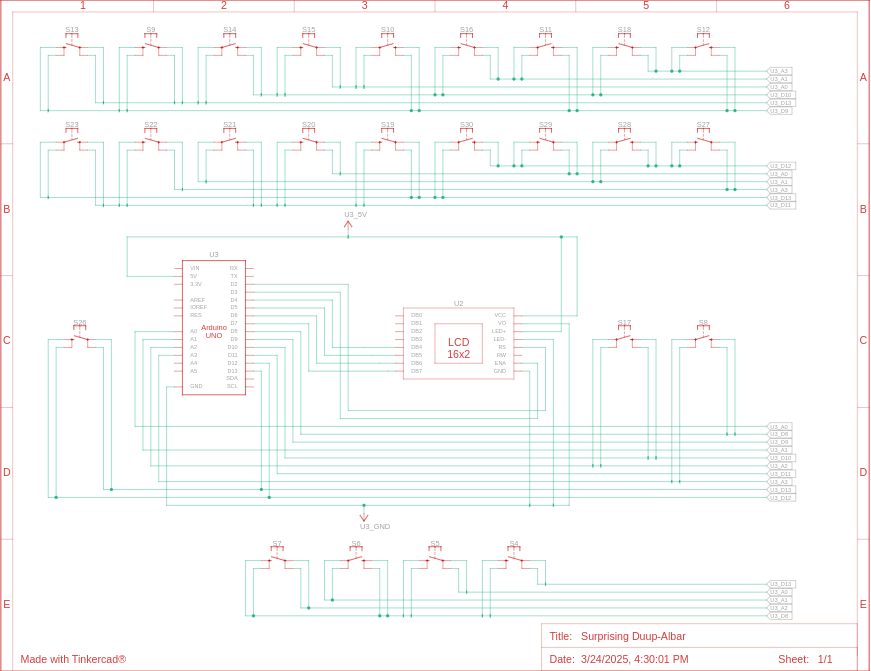
\includegraphics[width=0.5\textwidth]{figs/schematic.png}
    \caption{Schematic of Circuit.}
    \label{fig:circuit_schematic}
\end{figure}


\subsection{Hardware Circuit}
The hardware circuit of calculator,
\begin{figure}[htbp]
    \centering
    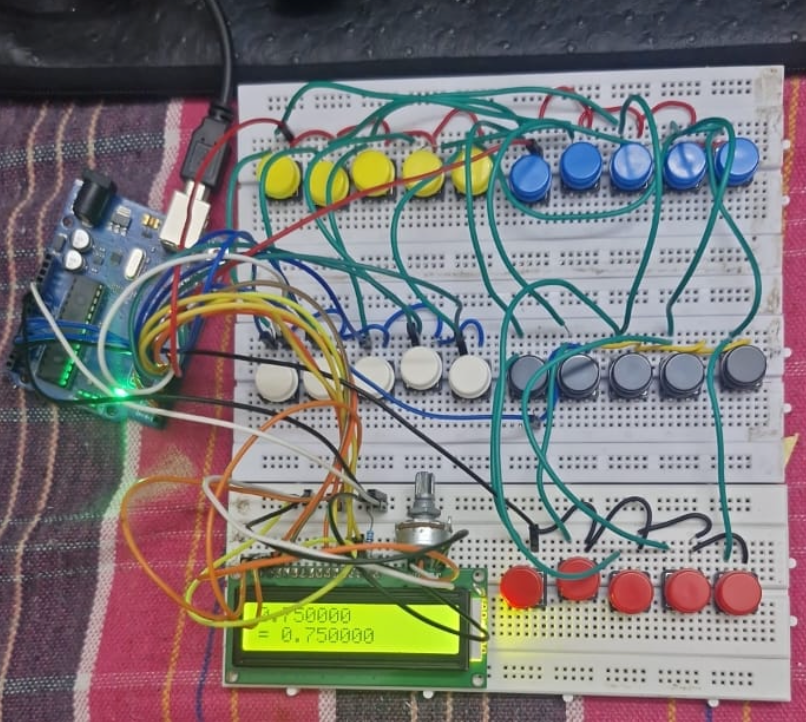
\includegraphics[width=0.5\textwidth]{figs/circuit.png}
    \caption{circuit}
    \label{fig:circuit}
\end{figure}


\appendices

\section{Runge--Kutta Method (RK4)}

\label{appendix:rk4}
The RK4 method is a numerical technique to solve
\begin{align}
\frac{dy}{dx} = f(x,y), \quad y(x_0)=y_0
\end{align}
with step size $h$. The next value is calculated as:
\begin{align}
y_{n+1} = y_n + \frac{1}{6}(k_1 + 2 k_2 + 2 k_3 + k_4)
\end{align}
where
\begin{align}
k_1 &= h f(x_n, y_n), \\
k_2 &= h f(x_n + h/2, y_n + k_1/2), \\
k_3 &= h f(x_n + h/2, y_n + k_2/2), \\
k_4 &= h f(x_n + h, y_n + k_3).
\end{align}

\subsubsection*{Quake III Algorithm}

\label{appendix:inv_sqrt}

The method obtains an initial approximation by manipulating the IEEE~754 floating-point representation of $x$, then refines it using Newton-Raphson iterations.

\begin{enumerate}
    \item Bit manipulation with a ``magic constant'' ($0x5f3759df$) produces an initial guess $y_0$.
    \item A single Newton--Raphson iteration dramatically improves accuracy.
    \item An optional second iteration yields nearly full precision. \\
\end{enumerate} 

\subsubsection*{Newton--Raphson Refinement}

We want to approximate
\begin{align} 
y = x^{-\frac{1}{2}}.
\end{align}

Define
\begin{align}
f(y) = \frac{1}{y^2} - x, \qquad f'(y) = -\frac{2}{y^3}.
\end{align}

Applying Newton--Raphson,
\begin{align}
y_{k+1} &= y_k - \frac{f(y_k)}{f'(y_k)} \\[6pt]
        &= y_k - \frac{\tfrac{1}{y_k^2} - x}{-\tfrac{2}{y_k^3}} \\[6pt]
        &= y_k + \frac{y_k}{2}\left(1 - x y_k^2 \right) \\[6pt]
        &= y_k \left(\tfrac{3}{2} - \tfrac{1}{2} x y_k^2\right).
\end{align}

Thus one Newton iteration is simply
\begin{align}
y \;\gets\; y \left( 1.5 - 0.5 \, x \, y^2 \right).
\end{align}



\begin{thebibliography}{00}

\bibitem{grewal2014}
B. S. Grewal, \textit{Higher Engineering Mathematics}, 43rd ed. New Delhi, India: Khanna Publishers, 2014.

\bibitem{GVVSharma}
G. V. V. Sharma,C Programming in Middle School

\bibitem{kreyszig2011}
E. Kreyszig, \textit{Advanced Engineering Mathematics}, 10th ed. Hoboken, NJ, USA: John Wiley \& Sons, 2011.

\bibitem{ncert12}
National Council of Educational Research and Training (NCERT), 
\textit{Mathematics: Textbook for Class XII}, Part 1 and 2, New Delhi, India: NCERT, 2006.

\end{thebibliography}

\end{document}


